\documentclass[UTF8]{article}
\usepackage{ctex}
\usepackage[a4paper, total={6in, 8in}]{geometry}
\usepackage{float}
\usepackage{underscore}
\usepackage{graphicx}
\usepackage{subfigure}
\usepackage{hyperref}
% \setCJKmainfont{Source Hans CJK}
\title{LSM-KV 项目报告}
\author{王雨杭 522021910183}
\date{2024年 5月 22日}

\usepackage{natbib}
\usepackage{graphicx}
\usepackage{enumitem}
\bibliographystyle{plain}

\begin{document}

\maketitle

\section{背景介绍}
LSM-KV 是一个基于日志结构合并树(Log-Structured Merge-tree,简称 LSM tree)的键值存储系统。LSM tree 是一种磁盘存储数据结构,用于处理大量随机写入的情况。它通过将随机写入转化为顺序写入,从而提高写入性能。
LSM-KV 项目的主要目标是实现一个高性能、可扩展的键值存储系统。它主要用于处理大数据应用,如搜索引擎、数据库和文件系统等,这些应用需要处理大量的数据写入和查询。同时,LSM tree也是RocksDB、LevelDB、HBase以及Prometheus等知名开源项目底层的存储引擎的数据结构,具有很高的学术和工业应用价值。

LSM-KV 的主要特点包括高性能(通过使用 LSM tree,LSM-KV 可以提供高性能的数据写入和查询)、可扩展性(LSM-KV 设计为可以在多台机器上分布式运行,从而处理大规模的数据)、支持多种数据类型(LSM-KV可以存储键值或复杂的数据类型,如列表、集合和哈希表)等,这些特点使 LSM-KV 成为处理大数据应用的理想选择。

对比B+树等持久化数据结构,LSM树具备一些专门为记录日志等磁盘写入密集型应用优化的特性,它的主要优势有写入效率高(LSM tree通过缓存写入操作并批量进行,可以显著减少磁盘I/O操作,从而提高写入效率)、高效的磁盘空间利用(LSM tree通过合并和压缩操作,可以有效地利用磁盘空间,减少数据冗余)、高并发性能好等,但在读取效率上存在一定的劣势。

在本项目之中,实现了基本的键值类型为{int, string} 的键值存储LSM树,支持GET、PUT、DELETE和SCAN操作,并实现了键值分离存储、支持GC、持久性和缓存、修改布隆过滤器大小等配置的特性。

% 这是一个对图片的引用, 图~\ref{fig:universe},以及参考文献~\cite{adams1995hitchhiker}。

% \begin{figure}[h!]
%   \centering
%   \includegraphics[width=0.5\textwidth]{universe}
%   \caption{The Universe}
%   \label{fig:universe}
% \end{figure}

\section{测试}

我的测试实现如下:在使用cache和Bloom Filter,使用Cache不使用Bloom Filter,两者都不使用三种情况下以及都使用,改变BloomFilter大小为1024 * i(i从1到15变化)字节几种情况,数据(value)大小分别为[10, 100, 1000, 10000]字节,开始GET,POST,DEL, SCAN前已有分别为[1000, 3000, 5000]组随机数据的情况下进行测试,每次测试随机GET 10000次取平均,PUT 1000次取平均, DEL 1000次取平均, SCAN 100次(范围随机)取平均测量耗时和吞吐量。
\subsection{性能测试}


\subsubsection{预期结果}
基于LSM tree的特性,应该表现出:
\begin{enumerate}
\item GET请求较慢,在使用缓存的情况下,会稍快
\item PUT和DEL请求较快,且由于DEL请求最坏只需要PUT一个小字符串,DEL应该比PUT更快
\item SCAN请求非常慢,因为要遍历每一层,与GET,PUT,DEL可能有数量级差距
\item 在触发合并时,PUT请求会显著变慢
\end{enumerate}

\subsubsection{常规分析}

\begin{enumerate}
    \item 对于Get、Put、Delete、Scan四种操作,在value大小为value\_size,预先插入键值对个数为prebuilt\_data\_num时,单次操作耗时如下表
    \begin{table}[H]
    \centering
    \begin{tabular}{|c|c|c|c|c|c|}
    \hline
    value\_size & prebuilt\_data\_num & Get & Put & Del & Scan \\
    \hline
    10 & 1000 & 1 & 4 & <1 & 24 \\
    100 & 1000 & 2 & 4 & <1 & 26 \\
    1000 & 1000 & 9 & 7 & <1 & 23 \\
    10000 & 1000 & 99 & 57 & <1 & 39 \\
    10 & 3000 & 5 & 11 & <1 & 868 \\
    100 & 3000 & 4 & 11 & <1 & 656 \\
    1000 & 3000 & 19 & 15 & <1 & 2684 \\
    10000 & 3000 & 140 & 59 & <1 & 18429 \\
    10 & 5000 & 6 & 15 & <1 & 1095 \\
    100 & 5000 & 8 & 13 & <1 & 1243 \\
    1000 & 5000 & 21 & 17 & <1 & 2804 \\
    10000 & 5000 & 147 & 62 & <1 & 21554 \\
    \hline
    \end{tabular}
    \caption{GET,PUT,DELETE,SCAN时延表(微秒)}
    \end{table}

    \item 在value大小为10、100、1000、10000字节, 在LSM之中预插入1000、3000、5000个数据,使用缓存和布隆过滤器,布隆过滤器大小为8KB的情况下,四种操作的吞吐如下表(key为8个字节,单位ops/s):
    \begin{table}[H]
    \centering
    \begin{tabular}{|c|c|c|c|c|c|}
    \hline
    value_size & prebuilt\_data\_num & Get & Put & Del & Scan \\
    \hline
    10 & 1000 & 5.22e+05 & 2.48e+05 & 2.74e+06 & 4.01e+04 \\
    100 & 1000 & 3.38e+05 & 2.26e+05 & 2.61e+06 & 3.71e+04 \\
    1000 & 1000 & 1.02e+05 & 1.29e+05 & 2.61e+06 & 4.18e+04 \\
    10000 & 1000 & 1.01e+04 & 1.74e+04 & 1.45e+06 & 2.53e+04 \\
    10 & 3000 & 1.69e+05 & 9.04e+04 & 2.46e+06 & 1.15e+03 \\
    100 & 3000 & 2.29e+05 & 8.38e+04 & 2.34e+06 & 1.52e+03 \\
    1000 & 3000 & 5.11e+04 & 6.28e+04 & 2.40e+06 & 3.73e+02 \\
    10000 & 3000 & 7.10e+03 & 1.68e+04 & 1.62e+06 & 5.43e+01 \\
    10 & 5000 & 1.54e+05 & 6.59e+04 & 2.38e+06 & 9.13e+02 \\
    100 & 5000 & 1.23e+05 & 7.16e+04 & 2.45e+06 & 8.04e+02 \\
    1000 & 5000 & 4.74e+04 & 5.63e+04 & 2.16e+06 & 3.57e+02 \\
    10000 & 5000 & 6.78e+03 & 1.61e+04 & 1.62e+06 & 4.64e+01 \\
    \hline
    \end{tabular}
    \caption{GET,PUT,DELETE,SCAN吞吐量表(ops/s)}
    \end{table}

典型的四种操作性能对比图如下~\ref{fig:性能对比图}:
\begin{figure}[ht]
    \centering
    \subfigure[]{
        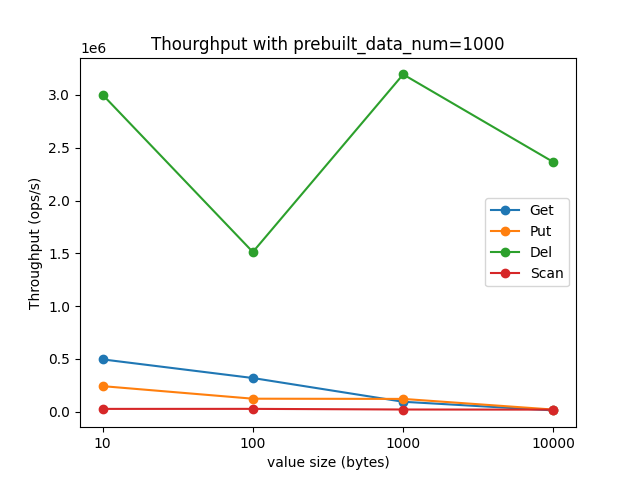
\includegraphics[width=0.3\textwidth]{../imgs/Thourghput with prebuilt_data_num=1000.png}
    }
    \subfigure[]{
        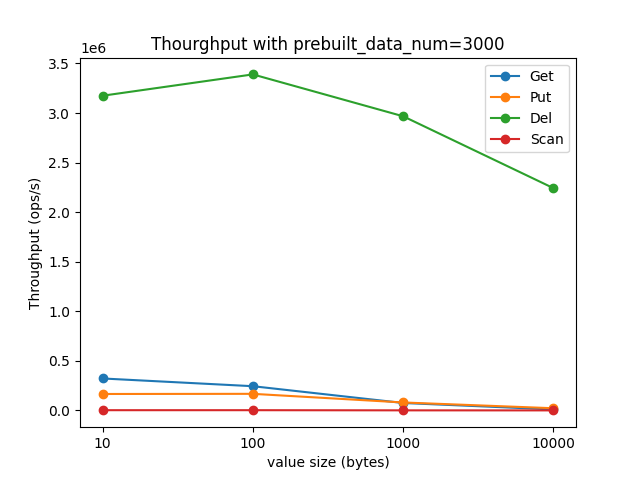
\includegraphics[width=0.3\textwidth]{../imgs/Thourghput with prebuilt_data_num=3000.png}
    }
    \subfigure[]{
        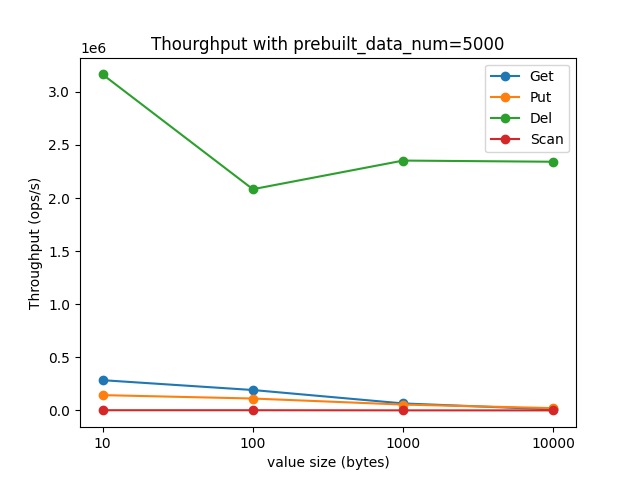
\includegraphics[width=0.3\textwidth]{../imgs/Thourghput with prebuilt_data_num=5000.png}
    }
    \caption{性能对比图}\label{fig:性能对比图}
\end{figure}
\\
分析两表和图~\ref{fig:性能对比图}可以得出以下结论:

\end{enumerate}
\begin{enumerate}
     \item 四种操作的速度从大到小为:DEL>GET>PUT>SCAN
     \item DEL速度非常快。这是因为在我的实现之中,DEL只在内存之中查找,最坏也只需要PUT一个短的value
     \item value较大时,GET操作退化的速度比PUT快,甚至到value\_size为10000个字节时,PUT比GET还快。这是因为GET需要多次query来确认key对应的value有效,而在存储的键值对都较长时,相关开销(例如,文件定位、取到验证用的magic和校验和)的开销远远超过了内存操作的开销,成为了开销的主体。这也验证了LSM结构在写上的优越性和读上效率不高的问题。
     \item SCAN操作也如预期的非常慢,与其他三种操作有数个数量级的差距。这是由于SCAN需要在sstable之中对每一层都进行查找归并,同时在vlog里面查找多个值。
\end{enumerate}

\subsubsection{索引缓存与Bloom Filter的效果测试}
对比下面三种情况GET操作的平均时延
\begin{enumerate}
    \item 内存中没有缓存SSTable的任何信息,从磁盘中访问SSTable的索引,在找到offset之后读取数据
    \item 内存中只缓存了SSTable的索引信息,通过二分查找从SSTable的索引中找到offset,并在磁盘中读取对应的值
    \item 内存中缓存SSTable的Bloom Filter和索引,先通过Bloom Filter判断一个键值是否可能在一个SSTable中,如果存在再利用二分查找,否则直接查看下一个SSTable的索引
\end{enumerate}
GET操作平均时延对比如下图~\ref{fig:三种情况下的GET平均时延随value大小变化}
\begin{figure}[h]
    \centering
    \subfigure[]{
        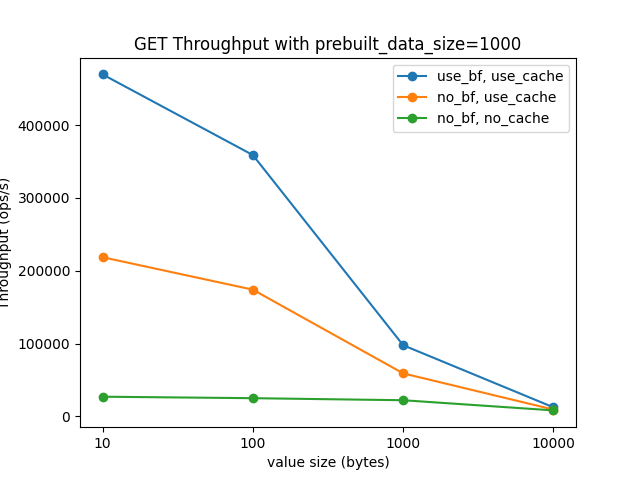
\includegraphics[width=0.3\textwidth]{../imgs/GET Throughput with prebuilt_data_size=1000}
    }
    \subfigure[]{
                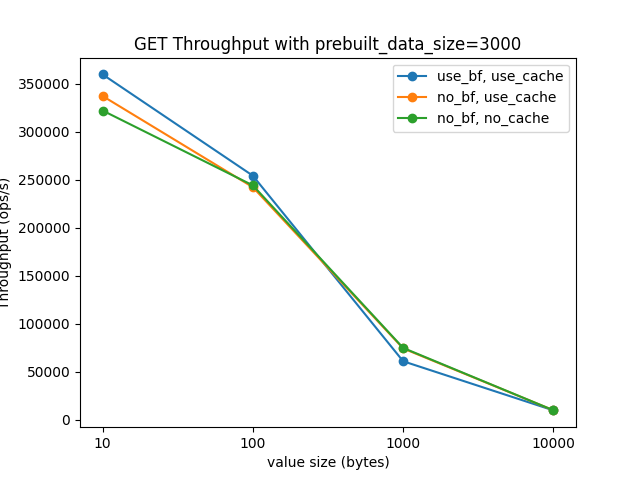
\includegraphics[width=0.3\textwidth]{../imgs/GET Throughput with prebuilt_data_size=3000}
    }
    \subfigure[]{
            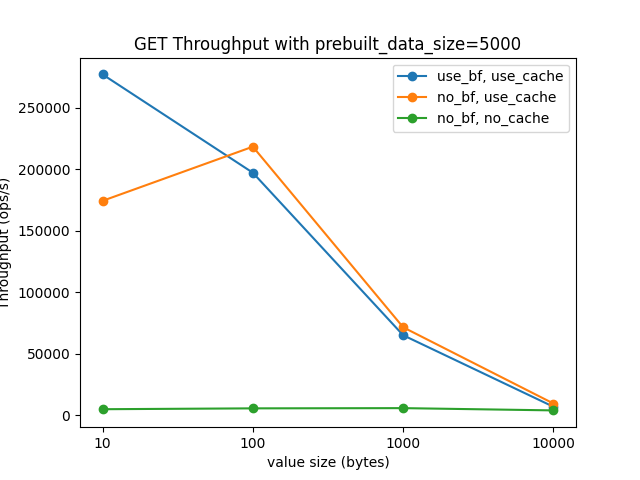
\includegraphics[width=0.3\textwidth]{../imgs/GET Throughput with prebuilt_data_size=5000}
    }
    \label{fig:三种情况下的GET平均时延随value大小变化}
\end{figure}
可以看到,在value大小较小,例如10个字节时,内存操作是影响GET平均时延的核心,因而缓存和布隆过滤器均有明显的加速效果,但在-Ofast优化下,效果也没有数量级的显著——约为20\%;而随着value变大,GET的平均时延转移到了磁盘操作,三种情况下时延趋于相同。

\subsubsection{Compaction的影响}
不断插入数据的情况下,PUT吞吐量随时间变化如图~\ref{fig:PUT吞吐量随时间变化图}:
\begin{figure}[h]
    \centering
    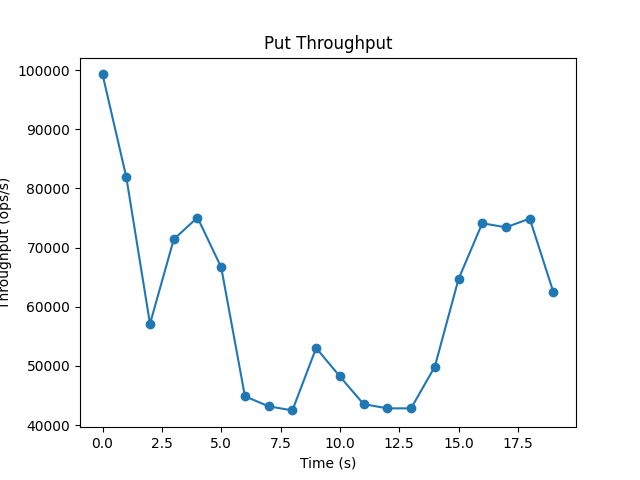
\includegraphics[width=0.8\textwidth]{../imgs/put_plot_8KB.png}
    \caption{PUT吞吐量随时间变化图}\label{fig:PUT吞吐量随时间变化图}
\end{figure}
可以发现,大趋势是put的吞吐量随时间增加而下降,但是在以秒计数的时间间隔之中,数值抖动明显,并且不断出现了局部吞吐量随时间增加而上升的情况。原因为:初始时数据较少,合并开销小,吞吐量非常高;而随着时间的增加,合并可能涉及的层数和SSTable个数也越来越多,合并的平均耗时增加。而抖动的原因是,新建一层的大合并(或者任意层数为n)的合并出现所需要的新增键值对个数随指数增长,在一秒的时间间隔内,已经无法保证合并的均匀性,在产生大合并的时间段内,吞吐量就低;而大合并结束后,吞吐量高,出现抖动。



\subsubsection{Bloom Filter 大小配置的影响}
理论上,Bloom Filter 过大会使得一个 SSTable 中索引数据较少,进而导致 SSTable 合并操作频繁;Bloom Filter 过小又会导致其 false positive 的几率过大,辅助查找的效果不好。

但在我的实验之中,Bloom Filter不同大小对PUT带来的效果不太明显,在不同大小Bloom Filter上运行20秒PUT,value\_size取100,吞吐量随时间变化的测试结果如图~\ref{fig:不同BloomFilter大小下的PUT}。

\begin{figure}[ht]
    \centering
    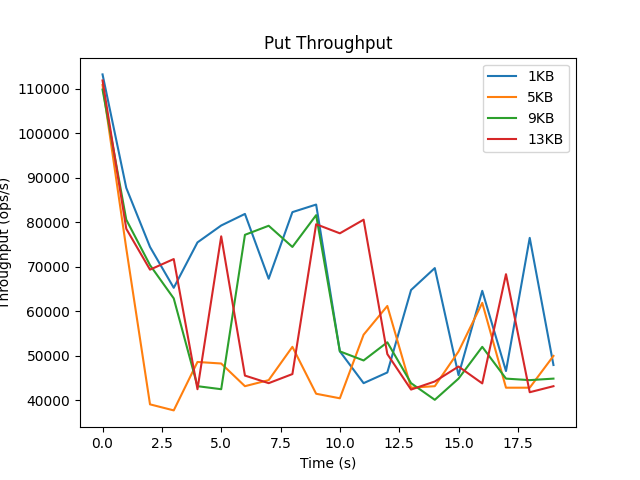
\includegraphics[width=0.5\textwidth]{../imgs/comparison.png}
    \caption{不同BloomFilter大小下的PUT}\label{fig:不同BloomFilter大小下的PUT}
\end{figure}

可以看到,曲线之间区别较小,可见在本次实验之中,PUT的性能决定点为vLog的写入部分,而BloomFilter大小的间接影响虽然不小,但相较vLog写入并不是最关键的。
而对于GET操作,我在不同value大小和预置数据大小上进行了测试,见图~\ref{fig:不同BloomFilter大小下的GET}。

\begin{figure}[H]
    \centering
    \subfigure[]{
        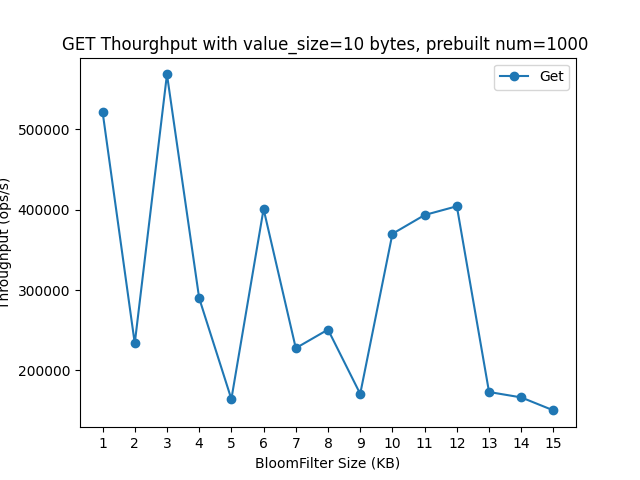
\includegraphics[width=0.45\textwidth]{../imgs/GET Thourghput with value_size=10 bytes, prebuilt num=1000 .png}
        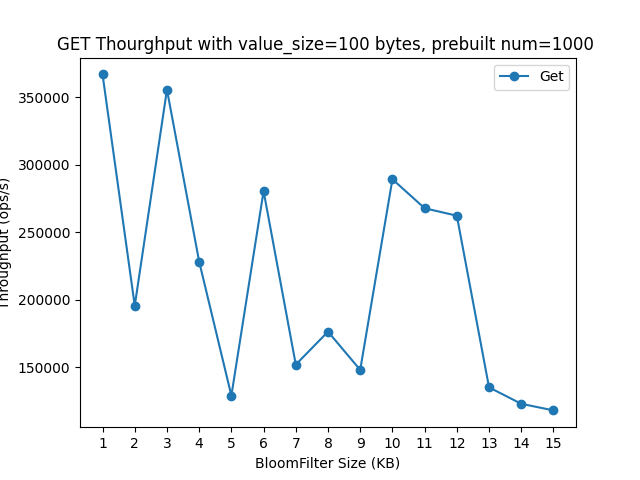
\includegraphics[width=0.45\textwidth]{../imgs/GET Thourghput with value_size=100 bytes, prebuilt num=1000 .png}
    }
    \subfigure[]{
        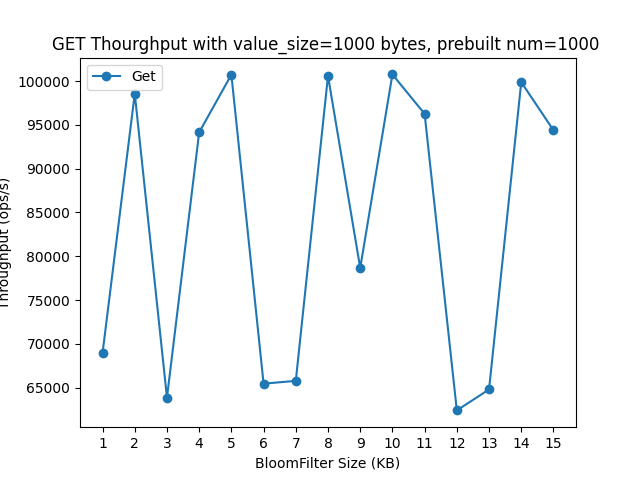
\includegraphics[width=0.45\textwidth]{../imgs/GET Thourghput with value_size=1000 bytes, prebuilt num=1000 .png}
        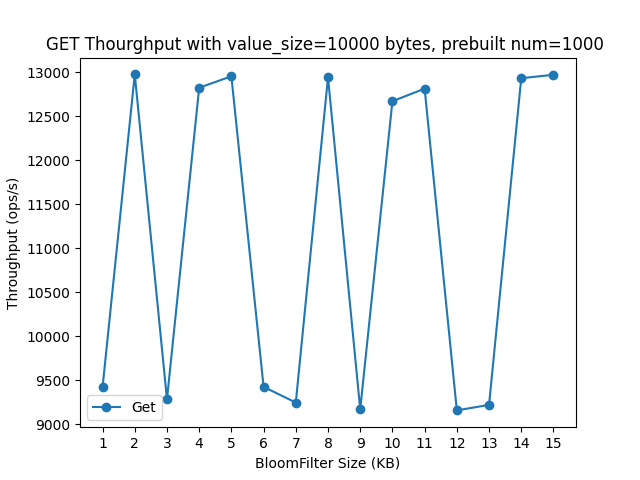
\includegraphics[width=0.45\textwidth]{../imgs/GET Thourghput with value_size=10000 bytes, prebuilt num=1000 .png}
    }
    \caption{不同BloomFilter大小下的GET}\label{fig:不同BloomFilter大小下的GET}
\end{figure}

可见整体上,决定GET吞吐量的是数据的value大小,这个参数对结果有数量级的影响。而在相同value大小下,在value大小较小时,BloomFilter的大小对性能的影响与理论较接近,适中的大小BloomFilter大小能够带来更好的性能表现;
但当value大小较大时,整体波动明显,BloomFilter的大小对性能的影响较小,性能瓶颈变成磁盘IO操作。
\section{结论}
在这个Project之中,我实现了一个具备较高鲁棒性和可用性的LSM键值存储系统,同时通过多种方法实现了较为完备的正确性和性能分析,性能表现符合预期,让我对这个project和对应的LSM树具备了更深刻的理解。

\section{致谢}
首先,我要感谢2022级软件工程专业的同学们,他们在我的学习和研究中提供了很多帮助和建议。特别是廖承凡同学,他在文档的理解交流过程中给予了我巨大的帮助。

其次,我要感谢张迟学长的mini-lsm项目\footnote{https://github.com/skyzh/mini-lsm},他对lsm的深入理解和剖析让我对如何改进这个项目有了许多新的想法。我还要感谢google的gtest项目\footnote{https://github.com/google/googletest},在这个框架的支持下,项目的测试和维护变得轻松不少。

感谢知乎的文章\footnote{https://zhuanlan.zhihu.com/p/415799237} ,让我对LSM树的实现有了更加清晰的认识;感谢GeeksforGeeks的一系列算法博客,让我对布隆过滤器和跳表都有了完整和清晰的认识;感谢Effective modern cpp、cppcon和cppreference,在这些书籍、视频和网站的帮助下,我了解了诸多项目中需要用的现代c++的语法知识。

\section{其他和建议}
\begin{enumerate}
    \item 困难与挑战:主要在于对modern cpp语法的不了解和c++文件操作带来的debug困难,这个project是一次很好的TDD(测试驱动开发)的实践,在不断地写单元测试、跑单元测试和回归测试的过程之中,我对每个子模块和整体的项目的正确性和架构如何解耦产生了许多新的认知。如何对持久化操作测试是有挑战的。
    \item bug: 印象最深的有两个:一个是传了vector的引用进一个函数,但在函数内部同时修改vector和使用vector的迭代器/引用——造成了重定位带来的迭代器失效问题;还有一个是在布隆过滤器的函数的实现里面捕获了一个悬垂指针。
    \item 吐槽:最后我的测试代码写得比实现代码都多了,感觉可以再给多一些测试框架,这是其一;助教的测试用例用"sssssss..."根本无法debug,这是其二;这个试验报告要测试的东西也太多了,我python脚本和c++测试文件又写了四五百行, 这是其三。
\end{enumerate}
\end{document}

